\chapter{Introduzione al corso}
\section{Il decimo problema di Hilbert}
Data un’equazione \textit{Diofantea} (polinomio con coefficienti interi posta uguale a 0) con qualsiasi numero di quantità incognite e con coefficienti numerici razionali interi, individuare un procedimento mediante il quale si possa determinare in un numero finito di operazioni se l’equazione è risolubile in razionali interi (Hilbert, Int. Congress of Mathematicians, Sorbona (Parigi), 8/8/1900).\\\\
\textbf{In termini moderni}: determinare un algoritmo per sapere se un’equazione Diofantea è risolubile. Non ci sono limiti al numero delle variabili ecc... , si possono quindi scrivere infinite equazioni Diofantee.
\begin{figure}[H]
	\centering
    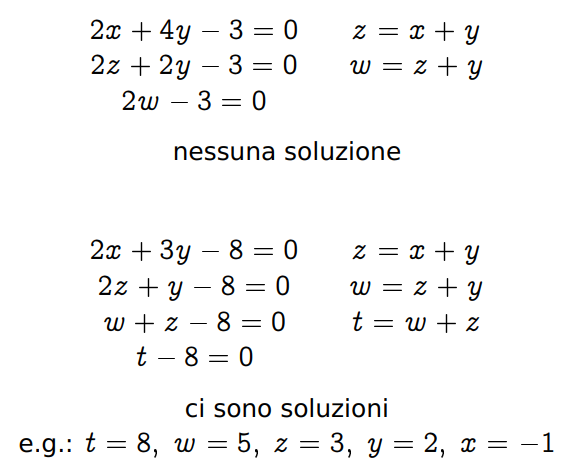
\includegraphics[width=8cm, keepaspectratio]{tesi_stile/img/dio1.png}
\end{figure}

\subsection{Teoria della Computabilità}
E se il 10th problema di Hilbert non avesse soluzione?\\
Dobbiamo rispondere alle domande:
\begin{enumerate}
    \item quali sono le funzioni per cui esiste un procedimento di calcolo effettivo?
    \item e quali quelle per cui un tale procedimento non esiste?
\end{enumerate}
Ma per rispondere alla domanda 2, è necessaria una \textbf{definizione formale di procedimento di calcolo effettivo}.\\\\
\textbf{Millennium prize problems (Millennium meeting Collège de France (Parigi), 24/5/2000)}\\
Il Clay Math. Institute (Boston) mette in palio 1.000.000\$ per chi risolve uno dei 7 problemi matematici più difficili.\\
Tra questi: \textbf{P vs. NP}
